\documentclass[tikz,border=0pt]{standalone}
\usepackage{amsmath,amssymb}
\DeclareMathSizes{10}{10}{7}{7}
\DeclareMathSizes{8}{8}{7}{7}
\usetikzlibrary{arrows.meta,shapes.geometric}
\definecolor{leftline}{RGB}{45,153,219}
\definecolor{leftfill}{RGB}{235,246,255}
\definecolor{midline}{RGB}{78,194,91}
\definecolor{midfill}{RGB}{236,250,236}
\definecolor{rightline}{RGB}{243,151,49}
\definecolor{rightfill}{RGB}{255,243,230}
\definecolor{trainline}{RGB}{137,84,198}
\definecolor{trainfill}{RGB}{249,243,255}
\definecolor{softblue}{RGB}{226,239,254}
\definecolor{softviolet}{RGB}{244,238,254}
\definecolor{softgreen}{RGB}{225,244,225}
\definecolor{softred}{RGB}{255,229,229}
\newcommand{\tinyfig}{\fontsize{7.2}{8.5}\selectfont}
\newcommand{\smallfig}{\fontsize{8}{9.2}\selectfont}
\newcommand{\headfig}{\fontsize{9}{10.5}\selectfont\bfseries}
\newcommand{\mathfig}{\fontsize{10}{11.5}\selectfont}
\begin{document}
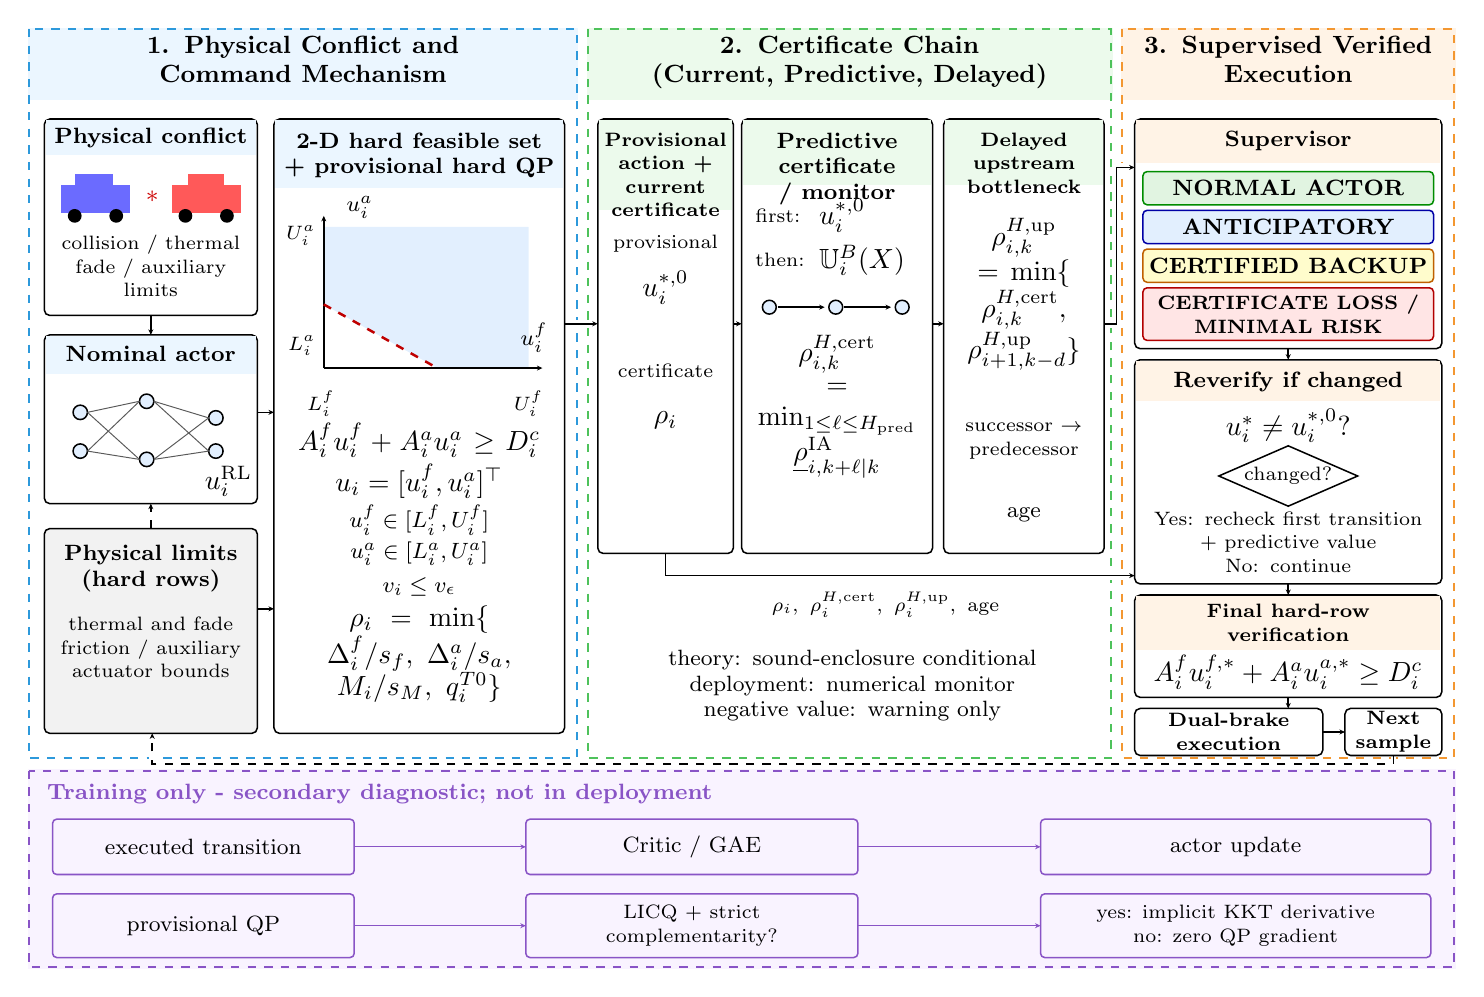
\begin{tikzpicture}[x=1pt,y=-1pt,line width=.55pt,
  mainflow/.style={draw=black,line width=.55pt,-{Stealth[length=2pt,width=1.8pt]}},
  trainingflow/.style={draw=trainline,line width=.45pt,-{Stealth[length=2pt,width=1.8pt]}},
  every node/.style={inner sep=0pt,outer sep=0pt}]
  % Fixed 516-pt print canvas. No global scale is used at integration width.
  \path[use as bounding box] (0,0) rectangle (516,340);
  \fill[leftfill] (0,0) rectangle (199,26);
  \fill[midfill] (202,0) rectangle (392,26);
  \fill[rightfill] (395,0) rectangle (516,26);
  \draw[leftline,dashed,line width=.7pt] (.5,.5) rectangle (198.5,264);
  \draw[midline,dashed,line width=.7pt] (202.5,.5) rectangle (391.5,264);
  \draw[rightline,dashed,line width=.7pt] (395.5,.5) rectangle (515.5,264);
  % Small white gateways keep signal arrows visually separate from dashed grouping borders.
  \fill[white] (197.7,105.5) rectangle (199.3,108.5);
  \fill[white] (201.7,105.5) rectangle (203.3,108.5);
  \fill[white] (390.7,105.5) rectangle (392.3,108.5);
  \fill[white] (394.7,49) rectangle (396.3,52);
  \fill[white] (390.7,196.5) rectangle (392.3,199.5);
  \fill[white] (394.7,196.5) rectangle (396.3,199.5);
  \fill[white] (492.5,263.3) rectangle (494.5,264.7);
  \fill[white] (44,263.3) rectangle (46,264.7);
  \node[anchor=north,align=center,font=\headfig,text width=190pt] at (99.5,3) {1. Physical Conflict and\\Command Mechanism};
  \node[anchor=north,align=center,font=\headfig,text width=184pt] at (297,3) {2. Certificate Chain\\(Current, Predictive, Delayed)};
  \node[anchor=north,align=center,font=\headfig,text width=116pt] at (455.5,3) {3. Supervised Verified\\Execution};

  % Section 1: opposed physics, nominal proposal, hard geometry and exact reserve.
  \draw[rounded corners=2pt] (6,33) rectangle (83,104);
  \fill[leftfill] (6.5,33.5) rectangle (82.5,46);
  \node[font=\smallfig\bfseries] at (44.5,40) {Physical conflict};
  \fill[blue!58] (12,57) rectangle (37,67);
  \fill[blue!58] (17,53) rectangle (31,58);
  \draw[fill=black] (17,68) circle (2.2);
  \draw[fill=black] (32,68) circle (2.2);
  \fill[red!65] (52,57) rectangle (77,67);
  \fill[red!65] (58,53) rectangle (71,58);
  \draw[fill=black] (57,68) circle (2.2);
  \draw[fill=black] (72,68) circle (2.2);
  \node[font=\headfig,text=red!80!black] at (45,61) {$\ast$};
  \node[anchor=north,align=center,font=\tinyfig,text width=73pt] at (44.5,75) {collision / thermal\\fade / auxiliary\\limits};

  \draw[rounded corners=2pt] (6,111) rectangle (83,172);
  \fill[leftfill] (6.5,111.5) rectangle (82.5,125);
  \node[font=\smallfig\bfseries] at (44.5,118) {Nominal actor};
  \foreach \p in {(19,139),(19,153),(43,135),(43,156),(68,141),(68,153)} {\draw[fill=softblue] \p circle (2.6);}
  \foreach \ya in {139,153} {\foreach \yb in {135,156} {\draw[black!65,line width=.35pt] (21.6,\ya) -- (40.4,\yb);}}
  \foreach \ya in {135,156} {\foreach \yb in {141,153} {\draw[black!65,line width=.35pt] (45.6,\ya) -- (65.4,\yb);}}
  \node[font=\mathfig,anchor=east] at (81,164) {$u_i^{\rm RL}$};

  \draw[rounded corners=2pt,fill=black!5] (6,181) rectangle (83,255);
  \node[anchor=north,align=center,font=\smallfig\bfseries,text width=73pt] at (44.5,187) {Physical limits\\(hard rows)};
  \node[anchor=north,align=center,font=\tinyfig,text width=72pt] at (44.5,213) {thermal and fade\\friction / auxiliary\\actuator bounds};
  \draw[mainflow] (44.5,104) -- (44.5,111);
  \draw[mainflow,dashed] (44.5,181) -- (44.5,172);

  \draw[rounded corners=2pt] (89,33) rectangle (194,255);
  \fill[leftfill] (89.5,33.5) rectangle (193.5,58);
  \node[anchor=north,align=center,font=\smallfig\bfseries,text width=101pt] at (141.5,38) {2-D hard feasible set\\+ provisional hard QP};
  \draw[mainflow] (83,139) -- (89,139);
  \draw[mainflow] (83,210) -- (89,210);
  % Correct northeast side of the coupled collision face is shaded.
  \fill[softblue] (107,72) -- (181,72) -- (181,123) -- (148,123) -- (107,100) -- cycle;
  \draw[mainflow] (107,123) -- (186,123);
  \draw[mainflow] (107,123) -- (107,68);
  \draw[red!75!black,dashed,line width=.9pt] (107,100) -- (148,123);
  \node[font=\tinyfig] at (106,136) {$L_i^f$};
  \node[font=\tinyfig] at (181,136) {$U_i^f$};
  \node[font=\tinyfig,anchor=east] at (104,75) {$U_i^a$};
  \node[font=\tinyfig,anchor=east] at (104,115) {$L_i^a$};
  \node[font=\smallfig] at (183,112) {$u_i^f$};
  \node[font=\smallfig] at (120,65) {$u_i^a$};
  \node[anchor=north,align=center,font=\mathfig,text width=102pt] at (141.5,143) {$A_i^fu_i^f+A_i^au_i^a\ge D_i^c$};
  \node[font=\mathfig] at (141.5,164) {$u_i=[u_i^f,u_i^a]^\top$};
  \node[font=\smallfig] at (141.5,178) {$u_i^f\in[L_i^f,U_i^f]$};
  \node[font=\smallfig] at (141.5,190) {$u_i^a\in[L_i^a,U_i^a]$};
  \node[font=\smallfig] at (141.5,202) {$v_i\le v_\epsilon$};
  \node[anchor=north,align=center,font=\mathfig,text width=101pt] at (141.5,209) {$\rho_i=\min\{$\\$\Delta_i^f/s_f,\ \Delta_i^a/s_a,$\\$M_i/s_M,\ q_i^{T0}\}$};

  % Section 2: the current two-output status and finite-horizon chain.
  \draw[rounded corners=2pt] (206,33) rectangle (255,190);
  \fill[midfill] (206.5,33.5) rectangle (254.5,66);
  \node[anchor=north,align=center,font=\tinyfig\bfseries,text width=44.5pt] at (230.5,38) {Provisional\\action + current\\certificate};
  \node[font=\tinyfig] at (230.5,78) {provisional};
  \node[font=\mathfig] at (230.5,94) {$u_i^{*,0}$};
  \node[font=\tinyfig] at (230.5,124) {certificate};
  \node[font=\mathfig] at (230.5,142) {$\rho_i$};
  \draw[mainflow] (194,107) -- (206,107);

  \draw[rounded corners=2pt] (258,33) rectangle (327,190);
  \fill[midfill] (258.5,33.5) rectangle (326.5,57);
  \node[anchor=north,align=center,font=\smallfig\bfseries,text width=66pt] at (292.5,38) {Predictive certificate\\/ monitor};
  \node[font=\tinyfig,anchor=west] at (263,68) {first:};
  \node[font=\mathfig,anchor=west] at (286,68) {$u_i^{*,0}$};
  \node[font=\tinyfig,anchor=west] at (263,84) {then:};
  \node[font=\mathfig,anchor=west] at (286,84) {$\mathbb U_i^B(X)$};
  \foreach \cx in {268,292,316} {\draw[fill=softblue] (\cx,101) circle (2.5);}
  \draw[mainflow] (271,101) -- (288,101);
  \draw[mainflow] (295,101) -- (312,101);
  \node[anchor=north,align=center,font=\mathfig,text width=66pt] at (292.5,111) {$\rho_{i,k}^{H,\mathrm{cert}}$\\$=\min_{1\le\ell\le H_{\rm pred}}$\\$\underline\rho_{i,k+\ell\mid k}^{\rm IA}$};
  \draw[mainflow] (255,107) -- (258,107);

  \draw[rounded corners=2pt] (331,33) rectangle (389,190);
  \fill[midfill] (331.5,33.5) rectangle (388.5,57);
  \node[anchor=north,align=center,font=\tinyfig\bfseries,text width=54pt] at (360,38) {Delayed upstream\\bottleneck};
  \node[anchor=north,align=center,font=\mathfig,text width=54pt] at (360,69) {$\rho_{i,k}^{H,\rm up}$\\$=\min\{$\\$\rho_{i,k}^{H,\rm cert},$\\$\rho_{i+1,k-d}^{H,\rm up}\}$};
  \node[anchor=north,align=center,font=\tinyfig,text width=54pt] at (360,143) {successor $\to$\\predecessor};
  \node[font=\smallfig] at (360,176) {age};
  \draw[mainflow] (327,107) -- (331,107);
  \draw[mainflow] (389,107) -- (393.5,107) -- (393.5,50.5) -- (400,50.5);
  \draw[mainflow] (230.5,190) -- (230.5,198) -- (400,198);
  \node[anchor=north,font=\tinyfig] at (310,204) {$\rho_i,\ \rho_i^{H,\rm cert},\ \rho_i^{H,\rm up},\ \mathrm{age}$};
  \node[anchor=north,align=center,font=\smallfig,text width=173pt] at (298,225) {theory: sound-enclosure conditional\\deployment: numerical monitor\\negative value: warning only};

  % Section 3: four-mode supervision, changed-action check and verified actuation.
  \draw[rounded corners=2pt] (400,33) rectangle (511,116);
  \fill[rightfill] (400.5,33.5) rectangle (510.5,49);
  \node[font=\smallfig\bfseries] at (455.5,41) {Supervisor};
  \filldraw[fill=softgreen,draw=green!55!black,rounded corners=1.5pt] (403,52) rectangle (508,64);
  \filldraw[fill=softblue,draw=blue!65!black,rounded corners=1.5pt] (403,66) rectangle (508,78);
  \filldraw[fill=yellow!20,draw=orange!75!black,rounded corners=1.5pt] (403,80) rectangle (508,92);
  \filldraw[fill=softred,draw=red!70!black,rounded corners=1.5pt] (403,94) rectangle (508,113);
  \node[font=\smallfig\bfseries] at (455.5,58) {NORMAL ACTOR};
  \node[font=\smallfig\bfseries] at (455.5,72) {ANTICIPATORY};
  \node[font=\smallfig\bfseries] at (455.5,86) {CERTIFIED BACKUP};
  \node[font=\tinyfig\bfseries,align=center] at (455.5,103.5) {CERTIFICATE LOSS /\\MINIMAL RISK};

  \draw[rounded corners=2pt] (400,120) rectangle (511,201);
  \fill[rightfill] (400.5,120.5) rectangle (510.5,135);
  \node[font=\smallfig\bfseries] at (455.5,128) {Reverify if changed};
  \node[font=\mathfig] at (455.5,144) {$u_i^*\ne u_i^{*,0}$?};
  \node[diamond,draw,aspect=2.3,inner sep=.6pt,font=\tinyfig] at (455.5,162) {changed?};
  \node[anchor=north,align=center,font=\tinyfig,text width=105pt] at (455.5,175) {Yes: recheck first transition\\+ predictive value\\No: continue};
  \draw[mainflow] (455.5,116) -- (455.5,120);
  \draw[mainflow] (455.5,201) -- (455.5,205);

  \draw[rounded corners=2pt] (400,205) rectangle (511,242);
  \fill[rightfill] (400.5,205.5) rectangle (510.5,225);
  \node[align=center,font=\tinyfig\bfseries] at (455.5,215) {Final hard-row\\verification};
  \node[font=\mathfig] at (455.5,233) {$A_i^fu_i^{f,*}+A_i^au_i^{a,*}\ge D_i^c$};
  \draw[mainflow] (455.5,242) -- (455.5,246);
  \draw[rounded corners=2pt] (400,246) rectangle (468,263);
  \draw[rounded corners=2pt] (476,246) rectangle (511,263);
  \node[align=center,font=\tinyfig\bfseries,text width=65pt] at (434,254.5) {Dual-brake execution};
  \node[align=center,font=\tinyfig\bfseries,text width=32pt] at (493.5,254.5) {Next\\sample};
  \draw[mainflow] (468,254.5) -- (476,254.5);
  \draw[mainflow,dashed] (493.5,263) -- (493.5,266) -- (45,266) -- (45,255);

  % Training is a clearly subordinate two-chain diagnostic strip.
  \fill[trainfill] (0,268) rectangle (516,340);
  \draw[trainline,dashed,line width=.7pt] (.5,268.5) rectangle (515.5,339.5);
  \node[anchor=west,font=\smallfig\bfseries,text=trainline] at (7,277) {Training only - secondary diagnostic; not in deployment};
  \draw[rounded corners=1.5pt,trainline] (9,286) rectangle (118,306);
  \draw[rounded corners=1.5pt,trainline] (180,286) rectangle (300,306);
  \draw[rounded corners=1.5pt,trainline] (366,286) rectangle (507,306);
  \node[font=\smallfig] at (63.5,296) {executed transition};
  \node[font=\smallfig] at (240,296) {Critic / GAE};
  \node[font=\smallfig] at (436.5,296) {actor update};
  \draw[trainingflow] (118,296) -- (180,296);
  \draw[trainingflow] (300,296) -- (366,296);
  \draw[rounded corners=1.5pt,trainline] (9,313) rectangle (118,336);
  \draw[rounded corners=1.5pt,trainline] (180,313) rectangle (300,336);
  \draw[rounded corners=1.5pt,trainline] (366,313) rectangle (507,336);
  \node[font=\smallfig] at (63.5,324.5) {provisional QP};
  \node[font=\tinyfig,align=center] at (240,324.5) {LICQ + strict\\complementarity?};
  \node[font=\tinyfig,align=center] at (436.5,324.5) {yes: implicit KKT derivative\\no: zero QP gradient};
  \draw[trainingflow] (118,324.5) -- (180,324.5);
  \draw[trainingflow] (300,324.5) -- (366,324.5);
\end{tikzpicture}
\end{document}
